\section{Introdução e Justificativa}
\label{sec:int}

Os avanços tecnológicos de sistemas distribuídos estão permitindo que as pessoas utilizem serviços com volumes massivos de dados para aplicações sensíveis a latência.
%
Essa situação é propícia a área de jogos massivos e tem atraído pesquisadores~\cite{mmo_analytic}.
%
O principal objetivo das pesquisas é reduzir a carga e o impacto a latência para o usuário final nos serviços~\cite{1417630}~\cite{6267019}~\cite{6063041}.
%
Reduzir a carga e impacto da latência em serviços para jogos massivos resultam em uma melhor experiência de jogabilidade aos usuários finais\cite{1417630}.



O mercado de jogos massivos multijogadores de interpretação (\textit{MMORPG}) vem crescendo desde 2012 \cite{new_york_times}, sendo no ano de 2016 um dos mais lucrativos\cite{statista_2016}. % ccm usar classe de acrônimos
%
A sua projeção para 2018 é que sejam arrecadados mais de 30 bilhões de dólares americanos com esta categoria de jogos \cite{statista_2018}, um aumento de 20\% a mais sobre o ano de 2016.



\ac{MMORPG} são jogos de interpretação de papéis massivos.
%
A principal característica desse estilo de jogo é a comunicação e representação virtual de um mundo fantasia na qual cada jogador pode interagir com objetos virtuais compartilhados ou tomar ações sobre outros de jogadores em tempo real, tendo como principais objetivos a resolução de problemas conforme a sua regra de \textit{design}, o desenvolvimento do personagem e a interação entre os jogadores\cite{video_game_technologies}.
%
Jogos \ac{MMORPG} são utilizados como negócio viável e lucrativo, a qual a experiência de uso do usuário final é um fator crítico para o sucesso.

Um jogo \ac{MMORPG} é arquitetado em 2 partes~\cite{mmo_analytic}:
\begin{itemize}
  \item \textbf{Serviço}: É o macroserviço que implementa as regras de negócio e requisitos do jogo.
  O serviço disponibiliza uma interface com ações possíveis ao cliente sobre algum protocolo de rede.
  \item \textbf{Cliente}: Cliente é a aplicação que realizará requisições com a interface do macroserviço, exibindo o estado de jogo de forma imersiva.
\end{itemize}

A maioria dos jogos \ac{MMORPG} disponíveis no mercado estão implementados sobre uma arquitetura que executa sobre diversos servidores, nos quais o desempenho destes servidores influencia na experiência do usuário final.
%
Modelar um sistema de alto desempenho torna-se um trabalho essencial para a satisfação do usuário final\cite{1417630}.
%
As ocorrências geradas por um sistema de baixo desempenho podem acarretar em frustração do usuário com o serviço e/ou aumento dos gastos com recurso computacional para manter o serviço.


\subsection{Ocorrências em serviços massivos}
\label{sec:ocorrencias}

Uma métrica popular para mensurar o desempenho de um serviço \ac{MMORPG} é o número de conexões\cite{1417630}.
%
Em geral, caso o serviço ultrapasse o limite para o qual este foi projetado, diversas falhas de conexão, problemas de lentidão ou dessincronização com o cliente podem ocorrer.
%
As ocorrências mais comuns são\cite{1417630}:

\begin{itemize}
  \item \textbf{Longo tempo de resposta aos clientes}: implica em uma qualidade insatisfatória de jogabilidade ao usuário ou até mesmo impossibilitando o uso do serviço.
  \item \textbf{Dessincronização com os clientes}: realiza reversão na aplicação. Reversão é definida pela situação onde uma requisição é solicitada ao servidor, um pré-processamento aparente é executado e essa requisição é negada, sendo necessário desfazer o pré-processamento aparente realizado ao cliente.
  \item \textbf{Problemas internos ao serviço}:  pode estar relacionada a diversos outros erros internos a implementação ou recursos internos do serviço (\textit{e.g.,} sobrecarga no banco de dados, gerenciamento lento do espaço ou inconsistências dentro do jogo perante a regra de negócios).
  \item \textbf{Falha de conexão entre o cliente e os microserviços}: causar a inacessibilidade do serviço ao usuário final.
\end{itemize}

Existem algumas causas comuns para essas as ocorrências descritas. Alguns problemas comuns para essas ocorrências\cite{1417630}:

\begin{itemize}
  \item \textbf{Baixo poder computacional do servidor}: poder computacional baixo para a qualidade de experiência do usuário final desejada.
  \item \textbf{Complexidade de algoritmos}: o serviço usa algoritmos de alta complexidade ou regras de negócios que demandam por um algoritmo complexo.
  \item \textbf{Limitado pela própria arquitetura}: está limitado diretamente pelo número de conexões, não suportando a carga recebida.
\end{itemize}

A área de desenvolvimento web compartilha várias ocorrências comums geradas por sobrecarga do serviço\cite{7830692}.
%
Em desenvolvimento web é comum utilizar a abordagem de microserviços para resolver o problema de sobrecarga, modularizando seu funcionamento em pedaços menores.
Da mesma forma, faz sentido modularizar um serviço \ac{MMORPG} em microserviços para suportar cargas menores.

\subsection{Arquiteturas de microserviços}

Entende-se por microserviço as aplicações que executam operações menores, da melhor forma possível, de um macroserviço\cite{stephenclarkewillson2017}.
%
Essas arquiteturas iniciam uma nova linha de desenvolvimento de aplicações preparadas para executar sobre nuvens computacionais, promovendo maior flexibilidade, escalabilidade, gerenciamento e desempenho, sendo a principal escolha de arquitetura de grandes empresas como Amazon, Netflix e LinkedIn\cite{7830692}\cite{7515686}.


A arquitetura Rudy~\cite{stephenclarkewillson2017}~\cite{matthiasrudy2011} (Figura~\ref{fig:rudy})
%ccm <-23
\begin{figure}[htb!]
  \caption{Arquitetura utilizada no jogo Tibia.}
  \label{fig:rudy}
  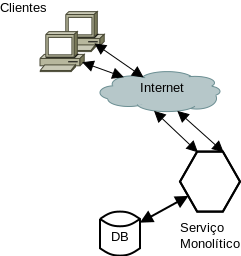
\includegraphics[width=5cm]{arquiteturas/monolitica.png}
  \centering

  Adaptado de:~\cite{stephenclarkewillson2017}
\end{figure}
%ccm <-24

\subsection{Justificativa}

A proposta de otimização das análises realizadas sobre as arquiteturas de microserviços para jogos massivos focada ao gerenciamento de mundos virtuais proposta pela literatura traz impacto direto a melhoria da qualidade de experiência ao usuário final e maior margem de lucro\cite{1417630}.
%
Por sua vez, proporcionando soluções com melhor garantia de sucesso sobre outras arquiteturas problemáticas.

%ccm justificar mais  def orma mais didática.
